\begin{table}[ht]
    \centering
    \begin{tabular}{c|c|c|c|c|c}
    \hline
    Dataset & \#$R_v$ & \#$R_e$ & Sum. $|R_v|$ & Sum. $|R_e|$ & Disk Usage\\
    \hline
    $LDBC10$ & 8 & 12 & 29,987,835 & 88,317,856 & 8.9G \\
    \hline
    $LDBC30$ & 8 & 12 & 88,789,833 & 278,652,443 & 28.0G\\
    \hline
    \revise{$LDBC100$} & 8 & 12 & 282,637,871 & 938,655,217 & 90.0G \\
    \hline
    \revise{$IMDB$} & 17 & 20 & 50,486,838 & 162,121,663 & 6.0G \\
    \hline
    \end{tabular}
    \caption{Statistics of the datasets. In detail, \#$R_v$ (resp.~\#$R_e$) is the number of vertex (resp.~edge) relations and Sum.~$|R_v|$ (Sum.~$|R_e|$) is the total number of tuples in vertex (resp.~edge) relations.
    \revise{Note that for the $IMDB$ datasets used in the graph database K\`uzu, we have manually designated the tables representing vertices and edges in the graph.}}
    \label{table:experiment-datasets}
\end{table}

\section{Evaluation}
\label{sec:evaluation}
% The experimental results are presented and analyzed in this section.
% In detail, experimental settings are introduced in Sec.~\ref{sec:experiment-settings}.
% Sec.~\ref{sec:experiment-e2e}-Sec.~\ref{sec:experiment-case-study} conduct the end-end experiments, test on queries with cycles, perform ablation studies, evaluate the optimization efficiency, test the efficiency of optimziations accross reltaional and graph queries, and evaluate the efficiency of the join order of the plans generated by \name, respectively.


%\enlargethispage{1em}

\subsection{Experimental Settings}
\label{sec:experiment-settings}

\noindent\textbf{Benchmarks.} Our experiments leverage two widely used benchmarks to assess system performance, as follows:
\begin{itemize}
    \item \textbf{LDBC SNB.} \revise{We use three datasets with scale factors of 10, 30, and 100, denoted as $LDBC10$, $LDBC30$, and $LDBC100$, respectively, generated by the official LDBC Data Generator. These datasets were chosen because they can be accommodated in the main memory of a single configured machine}.
    We select 10 queries from the LDBC Interactive workload for evaluation, denoted as $IC[1, \ldots, 9, 11, 12]$, with $10$, $13$, and $14$ excluded since they involve either pre-computation or shortest-path that are not supported.
    To accommodate queries containing variable-length paths~\cite{graindb}, we followed~\cite{graindb} to slightly modify them by separating each query into multiple individual queries with fixed-length paths. Each of these modified queries is denoted with a suffix ``-l'', where $l$ represents the length of the fixed-length path. In addition, we carefully designed two sets of queries for the comprehensiveness of evaluation, including (1) $QR[1\ldots 4]$ to test the effectiveness of heuristic rules \filterrule and \joinfuserule in \name, and (2) $QC[1\ldots 3]$, comprising three typical patterns with cycles including triangle, square, and 4-clique, to assess the efficiency of $\expandintersect$ introduced in \refsec{physical-operators}.
    \item \textbf{JOB.} The Join Order Benchmark (JOB)~\cite{job_snb} on Internet Movie Database (IMDB) is adopted. We select the variants marked with ``a'' of all JOB queries, referred to as $JOB[1\ldots 33]$, without loss of generality. These queries are primarily designed to test join order optimization, with each query containing an average of $8$ joins.
\end{itemize}
The details of the dataset statistics are summarized in Table \ref{table:experiment-datasets}.
We manually implement the queries using SQL/PGQ, which are presented in the artifact~\cite{artifact}.
%In addition, we adhered to the same procedures for data loading and graph index construction as those described in~\cite{graindb}.
Furthermore, we perform the \rgmapping process in a manner that allows the construction of the same graph index on the LDBC and JOB datasets used in GrainDB's experiments~\cite{graindb}.
\revise{Specifically, we store the data in DuckDB and construct both the EV-index and VE-index on potential edge relations, following the procedures described in GrainDB~\cite{graindb}. These indices are built on foreign keys and tables that depict many-to-many relationships}.
%The \rgmapping{s} are defined to ensure the effectiveness of the graph index defined in graindb.


\noindent\textbf{Compared Systems. }
%To ensure a fair comparison, \revise{All the following systems, except for K\`uzu, use DuckDB as the underlying relational execution engine, differing only in their adoption of the optimizer. Kùzu utilizes its own execution engine as a baseline of a graph database management system (GDBMS)}.
\revise{To ensure a fair comparison, all the following systems, except for K\`uzu, use DuckDB as the underlying relational execution engine, differing only in their adoption of the optimizer. DuckDB v0.9.2 is used in the experiments. Since GrainDB was originally implemented on an older version of DuckDB, we have reimplemented it on DuckDB v0.9.2, which offers improved performance over the original version. %Additionally, because the plans generated by Umbra might include multiway joins, we implemented multiway joins in DuckDB using the Leapfrog Trie Join algorithm (\todo{add references}).
K\`uzu utilizes its own execution engine (v0.4.2) as a baseline of a graph database management system (GDBMS).}

\begin{itemize}
\item DuckDB~\cite{duckdb}: This system optimizes queries using the graph-agnostic approach, leveraging DuckDB's built-in optimizer as described in \refsec{relational-only}. It serves as the naive baseline for extending a relational database system to support \spjm.

\item GrainDB~\cite{graindb}: This system uses same optimizer as DuckDB but employs the graph index (\refsec{graph-index}) for query execution. It acts as the baseline to demonstrate that solely using graph index is insufficient for optimizing \spjm.

%\item \relgohash: This system optimizes queries using the graph-agnostic optimizer introduced in \refsec{converged}, without leveraging the graph index for query execution. It serves as the baseline to showcase that, even in the absence of a graph index, the converged optimizer can generate efficient plans with improved join orders by utilizing graph-optimization techniques.

\item Umbra~\cite{umbra2020vldb,umbra2020cidr}: \revise{
    This system is equipped with an advanced hybrid optimizer capable of generating worst-case optimal join plans. We obtained the Umbra executable from the authors and configured its parameters according to their recommendations for computing the execution plan. The execution plan is then executed on DuckDB\footnote{Notably, all Umbra's plans for the benchmark queries exclude the multiway-join operator, allowing for direct transformation into DuckDB’s runtime.}, utilizing the graph index when applicable, as done in GrainDB.. This helps demonstrate that even with an advanced relational optimizer and the addition of a graph index, it can still fall short in optimizing \spjm.
    }

\item \name: This system optimizes queries using the converged optimizer presented in \refsec{converged} and utilizes the graph index for query execution. It demonstrates the full range of techniques introduced in this paper. There are some variants
of \name~ for verifying the effectiveness of the proposed techniques, which will be introduced in the corresponding experiments.

\item K\`uzu~\cite{jin2023cidr}:
\revise{
    This system is an embeddable GDBMS that adopts the property graph data model. We use it as a baseline to compare the performance gap between \name on relational databases and native graph databases.
}
\end{itemize}

%\revise{Please note that DuckDB v0.9.2 is used in the experiments. Since GrainDB was originally implemented on an older version of DuckDB, we have reimplemented it on DuckDB v0.9.2 to ensure a fair comparison. Additionally, because the plans generated by Umbra might include multiway joins, we implemented multiway joins in DuckDB using the Leapfrog Trie Join algorithm.
%The version of K\`uzu used in the experiments is v0.4.2}.

%We compare \name against two state-of-art baseline systems: DuckDB~\cite{duckdb} as a representative of $Rel$ optimizers, and GrainDB~\cite{graindb} as a representative of $Rel^+$ optimizers.
%For fair comparison, we use DuckDB as the underlying relational engine for all compared systems.
%To facilitate the evaluation of further optimizations brought by GrainDB and \name,
%we integrate pre-built graph indices into the backend storage, and implement the \intersect~ operator with worst-case optimal join implementation in the backend DuckDB engine.
%In this case, all the plans generated by different optimizers in the compared systems can be executed on the same backend.
%Then the comparison between these systems lies in their optimizers: DuckDB's optimizer will not consider the graph indices in query optimization, such that all queries will be executed with hash joins (even when graph indices are available);
%GrainDB will leverage the graph indices, and replace some hash joins with sip joins or merge sip joins to improve the efficiency of the plans;
%and for \name, in addition to graph indices, it will further consider converged optimizations across graph and relational query semantics, and leverage the optimized implementation for intersect operators.
%For simplicity, in the following, when there is no ambiguity, the optimizers of DuckDB and GrainDB are shortened to DuckDB and GrainDB, respectively.

% We compare \name against two state-of-art baseline systems: DuckDB~\cite{duckdb} as a representative of $Rel$ optimizers, and GrainDB~\cite{graindb} as a representative of $Rel^+$ optimizers.
% For fair comparison, we use the backend of GrainDB, which integrated pre-built graph indices, as a common backend for all compared systems.
% As the latest released GrainDB is based on an old version of DuckDB, which may miss out the latest optimizations developed in DuckDB, we upgrade the integrated DuckDB (in GrainDB) to v0.9.2.
% Meanwhile, when compared with DuckDB, we also use the same version.
% The difference between DuckDB and GrainDB lies in the optimizer, where DuckDB's optimizer will not consider the graph indices in query optimization, such that all queries will be executed with hash joins (even when graph indices are available),
%  while GrainDB will leverage the graph indices, and replace some hash joins with sip joins (or merge sip joins) to improve the efficiency of the plans.
% For \name, we further implement extend-intersect operators in the backend (as discussed in \refsec{physical-operators}), which not only leverage the graph indices, but also has an optimized worst-case optimal join implementation for \intersect.
% Therefore, all the generate plans can be executed on the same backend, and the efficiency of the plans obtained by varied optimizers can be compared fairly.
% Note that codegen techniques can be employed to facilitate the transformation of the physical plans into executable code.
% For simplicity, in the following, when there is no ambiguity, the optimizers of DuckDB and GrainDB are shortened to DuckDB and GrainDB, respectively.

\noindent\textbf{Configurations. }
Our experiments were conducted on a server equipped with an Intel Xeon E5-2682 CPU running at 2.50GHz and \revise{256GB} of RAM, with parallelism restricted to a single thread.
%We use the latest version of DuckDB as the common relational execution engine.
%To build the graph indices, we adhered to the same procedures for data processing and graph index construction as outlined in~\cite{graindb}.
%Note that codegen techniques can be employed to facilitate the transformation of the physical plans into executable code.
For a comprehensive performance analysis, each query from the LDBC benchmark was run 50 times using the official parameters, while each query from the JOB benchmark was executed 10 times. We report the average time cost for each query to mitigate potential biases.
We imposed a timeout limit of 10 minutes for each query, and queries that fail to finish within the limit are marked as \ot.

%\enlargethispage{1em}

\subsection{Micro Benchmarks on RelGo}
\label{sec:experiment-opt}
In this subsection, we conducted three micro benchmarks to evaluate the effectiveness of \name,
including assessing the efficiency of the optimizer, testing its advanced optimization strategies, and examining its effectiveness in optimizing join order.

\noindent\textbf{Optimization Efficiency Evaluation.}
First, we assessed the optimization efficiency by comparing \name with GrainDB\cite{graindb}.
%Specifically, \name employs a graph-aware optimizer, which explores in a significantly narrowed search space as analyzed in \refsec{compare-search-space}.
%In contrast, GrainDB utilizes graph-agnostic optimizer but generally employs a greedy optimization approach.
We compared the optimization time of \name and GrainDB, and also evaluated the execution time for their optimized plans as a measure of the plan quality.
We considered end-to-end time as optimization time plus execution time.
We randomly selected two subsets of the LDBC and JOB queries, and conducted the experiments on $LDBC30$ and IMDB datasets respectively.

The results, shown in Fig.~\ref{fig:exp-optimization}, reveal that \name significantly outperforms GrainDB in terms end-to-end time.
Specifically, \name achieves an average speedup of \revise{$7.5\times$} over GrainDB on the $LDBC30$ dataset and \revise{$3.8\times$} on the IMDB dataset.
However, it is worth noting that \name incurs a slightly higher optimization cost compared to GrainDB. Although \name theoretically has a narrower search space, as analyzed in \refsec{compare-search-space}, GrainDB benefits from DuckDB's optimizer, which includes very aggressive pruning strategies.
%This outcome is expected to some extent, given GrainDB's design focuses on greedy, faster optimization methods.

Despite the slightly higher optimization cost, the quality of the optimized plans generated by \name is generally superior to those produced by GrainDB. This is evident in the results of execution time, where \name outperforms GrainDB by an average of \revise{$9.7\times$} on the $LDBC30$ dataset and \revise{$4.3\times$} on the IMDB dataset. %When considering the total time cost, which includes both optimization and execution, \name still achieves an average speedup of $6.5\times$ over GrainDB on the $LDBC30$ dataset and $2.2\times$ on the IMDB dataset.
%This gap could be more obvious when the dataset scales up (comparing $LDBC10$ and $LDBC30$), since the optimization time cost is fixed, but a better plan will achieve more efficiency when the dataset scales up.
%These findings suggest that \name's optimization cost is justified, as it generates high-quality plans that are more efficient than those optimized by GrainDB in execution.

For fair comparison, in the subsequent experiments, we evaluate the efficiency of different systems using the end-to-end time.

\comment{
\textcolor{blue}{
First, we assessed the optimization efficiency by comparing \name with Apache Calcite\cite{calcite} and GrainDB\cite{graindb}.
Calcite, utilizing  a volcano-style query optimizer that is graph-agnostic, explores the search space to determine the most efficient plan.
In contrast, \name employs a graph-aware optimizer, which explores in a significantly narrowed search space as analyzed in \refsec{compare-search-space}.
To validate our theoretical findings, we conducted comparisons between \name and Calcite.
To broaden our analysis, we also compared \name against GrainDB, another graph-agnostic optimizer but generally employs a greedy optimization approach.
We compared the optimization time of \name, Calcite, and GrainDB, and also evaluated the execution time for their optimized query plans as a measure of the plan quality.
We select two subsets of the LDBC and JOB queries without loss of generality, and conduct the experiments on $LDBC30$ and IMDB datasets respectively.
The results are shown in Fig.~\ref{fig:exp-optimization}.
}

The experimental results reveal \name is significantly faster in optimization compared to Calcite.
Furthermore, the execution times of the query plans optimized by \name are either faster or comparable to those produced by Calcite.
For example, in the LDBC queries ($IC[7]$ excluded) shown in \reffig{exp-opt-ldbc}, the optimization time cost of \name is about two orders of magnitude faster than that of Calcite, and the execution time of the plans optimized by \name is more than 52.0$\times$ faster, on average.
It is worth noting that for query $IC[7]$ and all queries in JOB, Calcite cannot even finish the optimization within the timeout limit (thus we omit the results of Calcite in \reffig{exp-opt-job}).
On the contrary, \name shows an efficient optimization process for these queries.
This stark contrast accentuates \name's capability to efficiently generate optimized plans, confirming the effectiveness of its graph-aware optimizer in reducing the search space and improving the optimization efficiency.


Then we move to the comparison between \name with GrainDB. Compared with GrainDB, \name demonstrates a slightly higher optimization cost. This outcome is expected to some extent, given GrainDB's design focuses on greedy, faster optimization methods.
Nevertheless, the quality of \name's optimized plans are usually superior. This can be observed in the execution time results, where \name outperforms GrainDB by $9.5\times$ and $2.8\times$ on average on the $LDBC30$ and IMDB datasets, respectively.
For the total time cost of optimization and execution, \name still achieves $6.5\times$ and $2.2\times$ speedup over GrainDB on average, on the $LDBC30$ and IMDB datasets, respectively.
%This gap could be more obvious when the dataset scales up (comparing $LDBC10$ and $LDBC30$), since the optimization time cost is fixed, but a better plan will achieve more efficiency when the dataset scales up.
These findings suggest that \name's optimization cost is justified, as it generates high-quality plans that are more efficient than those optimized by GrainDB in execution.

To ensure a fair comparison, in the subsequent experiments, we evaluated the efficiency of different systems by considering the total time for both optimization and execution.
}

\begin{figure}[ht]
    \centering
    \begin{subfigure}[b]{\linewidth}
        \centering
        
\includegraphics[width=\linewidth]{./figures/exp/opt_exe_legends.pdf}
        \label{fig:exp-opt-legends}
        \vspace*{-2.5ex}
    \end{subfigure}
    \begin{subfigure}[b]{0.48\linewidth}
        \centering
        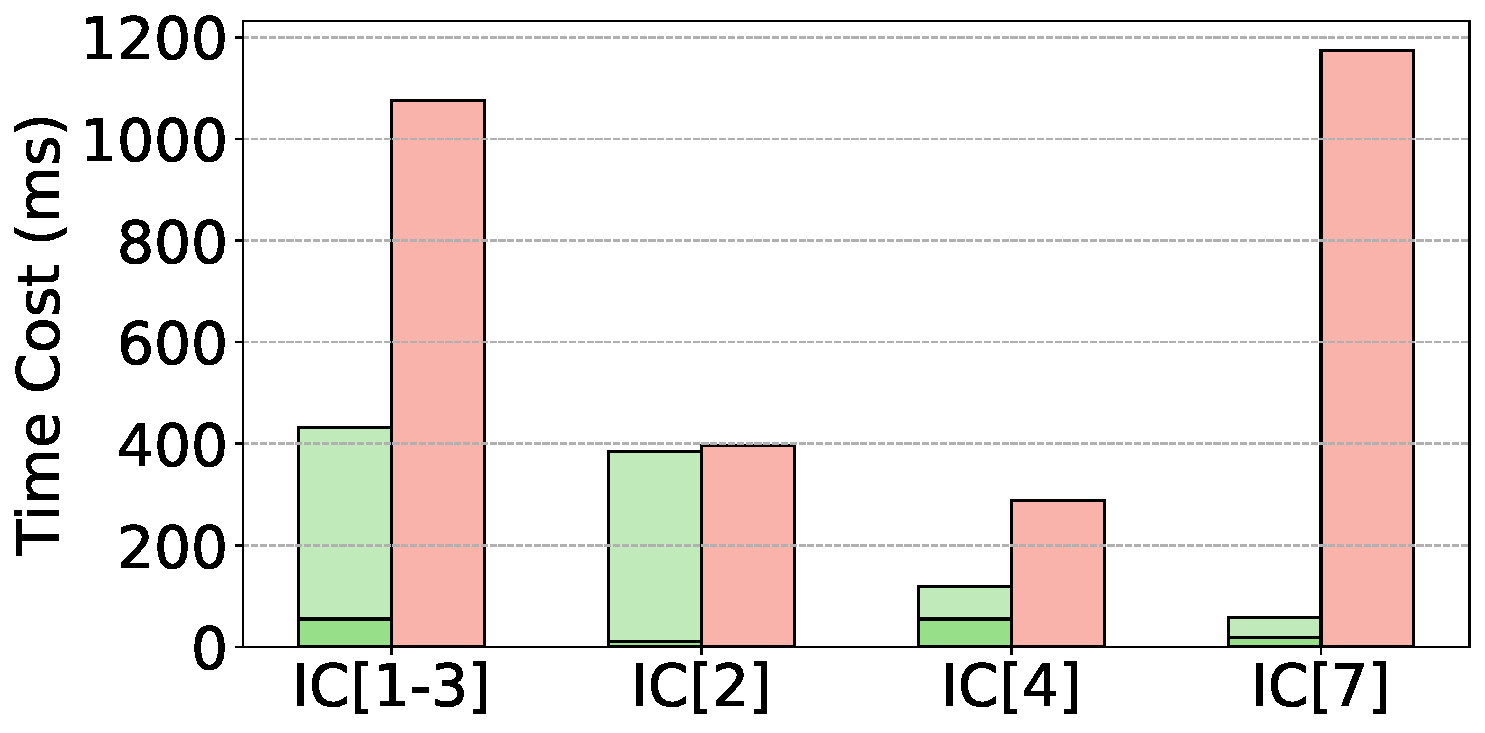
\includegraphics[width=\linewidth]{./figures/exp/opt_exe_ldbc.pdf}
        \vspace{-1.5em}
        \caption{End-to-End Time on $LDBC30$.}
        \label{fig:exp-opt-ldbc}
    \end{subfigure}
    \begin{subfigure}[b]{0.48\linewidth}
        \centering
        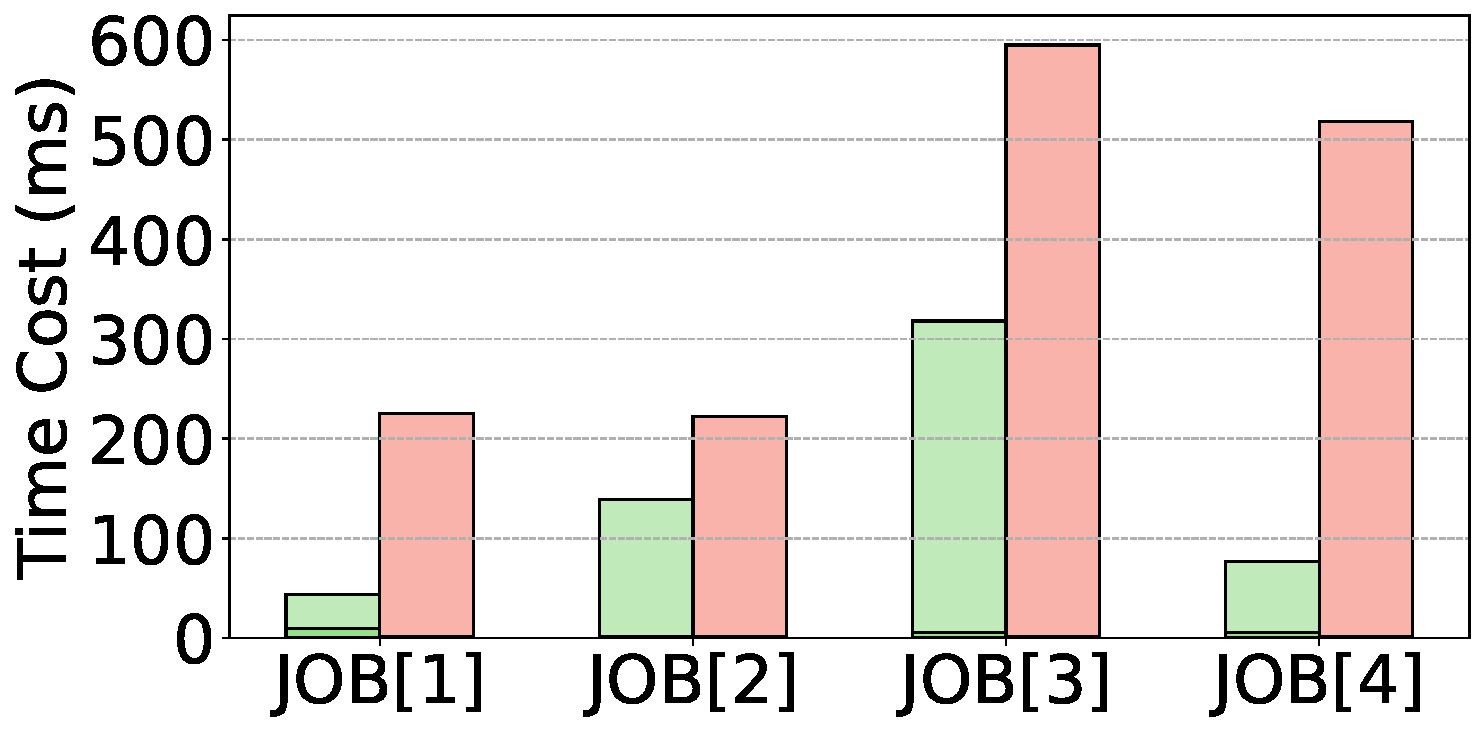
\includegraphics[width=\linewidth]{./figures/exp/opt_exe_job.pdf}
        \vspace{-1.5em}
        \caption{End-to-End Time on IMDB.}
        \label{fig:exp-opt-job}
    \end{subfigure}
    \caption{Experiments on optimization and execution cost}
    \label{fig:exp-optimization}
\end{figure}

% In the experiments, optimizing all the queries with \name can be finished in 10 minutes, while optimizing some queries with Calcite exceeds the 10-minute limit.
% For example, when JOB benchmark is utilized, the time cost of optimizing all the queries with Calcite is longer than 10 minutes.
% As shown in Fig.~\ref{fig:exp-optimization}, \name is much more efficient than Calcite in optimizing queries, and it is consistent with the conclusions obtained in Sec.~\ref{sec:theoretical-analysis}.
% That is, \name is exponentially faster than Calcite in query optimization.
% For instance, when IC5-1 is queried on $LDBC30$, the time cost of query optimization with \name can be more than $10^4\times$ faster than that of Calcite.

% Besides, the optimization time cost of \name is similar on $LDBC10$ and $LDBC30$, and so is Calcite.
% The reason is that the time required for optimization is not significantly associated with the scale of the dataset; instead, it is related to the relative cardinalities among the different tables.
% The relative cardinalities in LDBC datasets of different scales are consistent, therefore the optimization time is similar.

\begin{figure}[ht]
    \vspace{-1em}
    \centering
    \begin{subfigure}[b]{.45\linewidth}
        \centering
        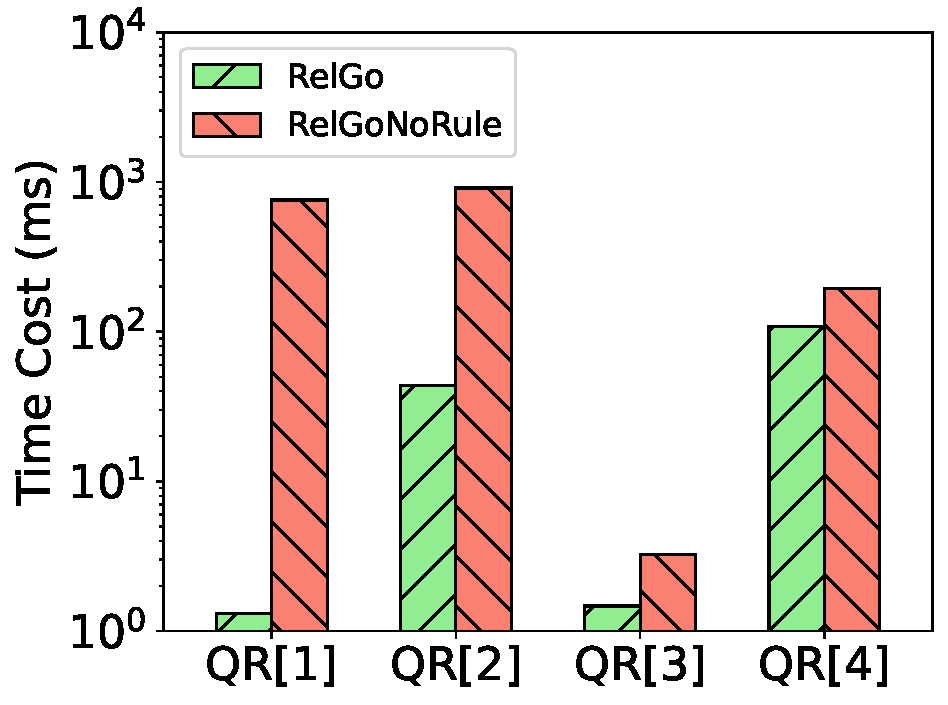
\includegraphics[width=\linewidth]{./figures/exp/filter_sf10.pdf}
        \vspace{-1.5em}
        \caption{Time Cost on $LDBC10$.}
        \label{fig:exp-filter-sf10}
    \end{subfigure}
    \begin{subfigure}[b]{0.45\linewidth}
        \centering
        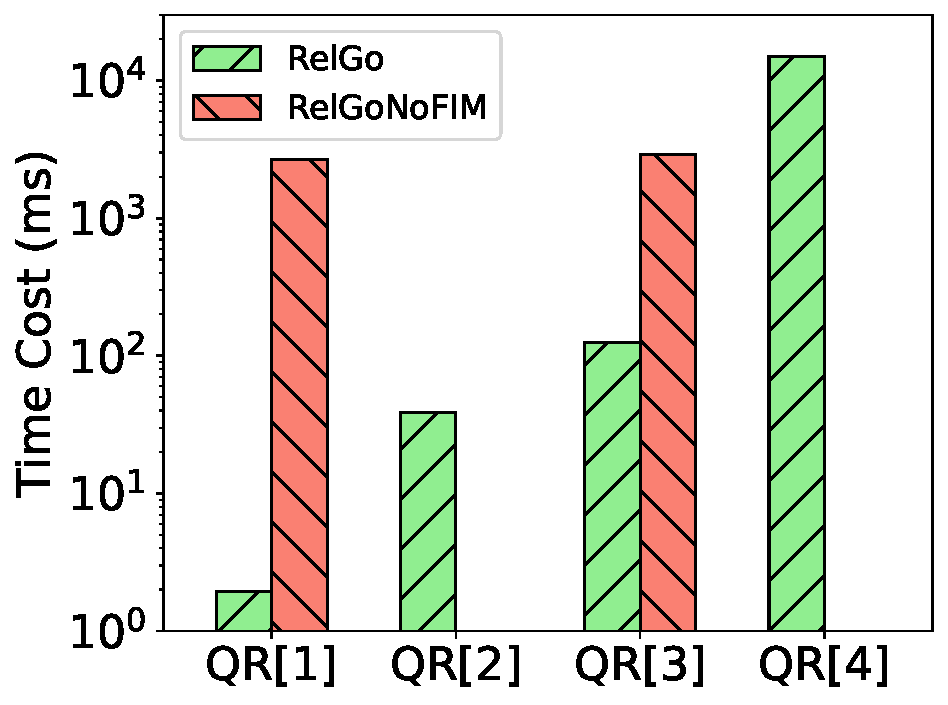
\includegraphics[width=\linewidth]{./figures/exp/filter_sf30.pdf}
        \vspace{-1.5em}
        \caption{Time Cost on $LDBC30$.}
        \label{fig:exp-filter-sf30}
    \end{subfigure}
    \caption{Efficiency comparison of \name and \relgonofi}
    \label{fig:exp-filter}
\end{figure}

\begin{figure}[ht]
    \vspace{-1em}
    \centering
    \begin{subfigure}[b]{.45\linewidth}
        \centering
        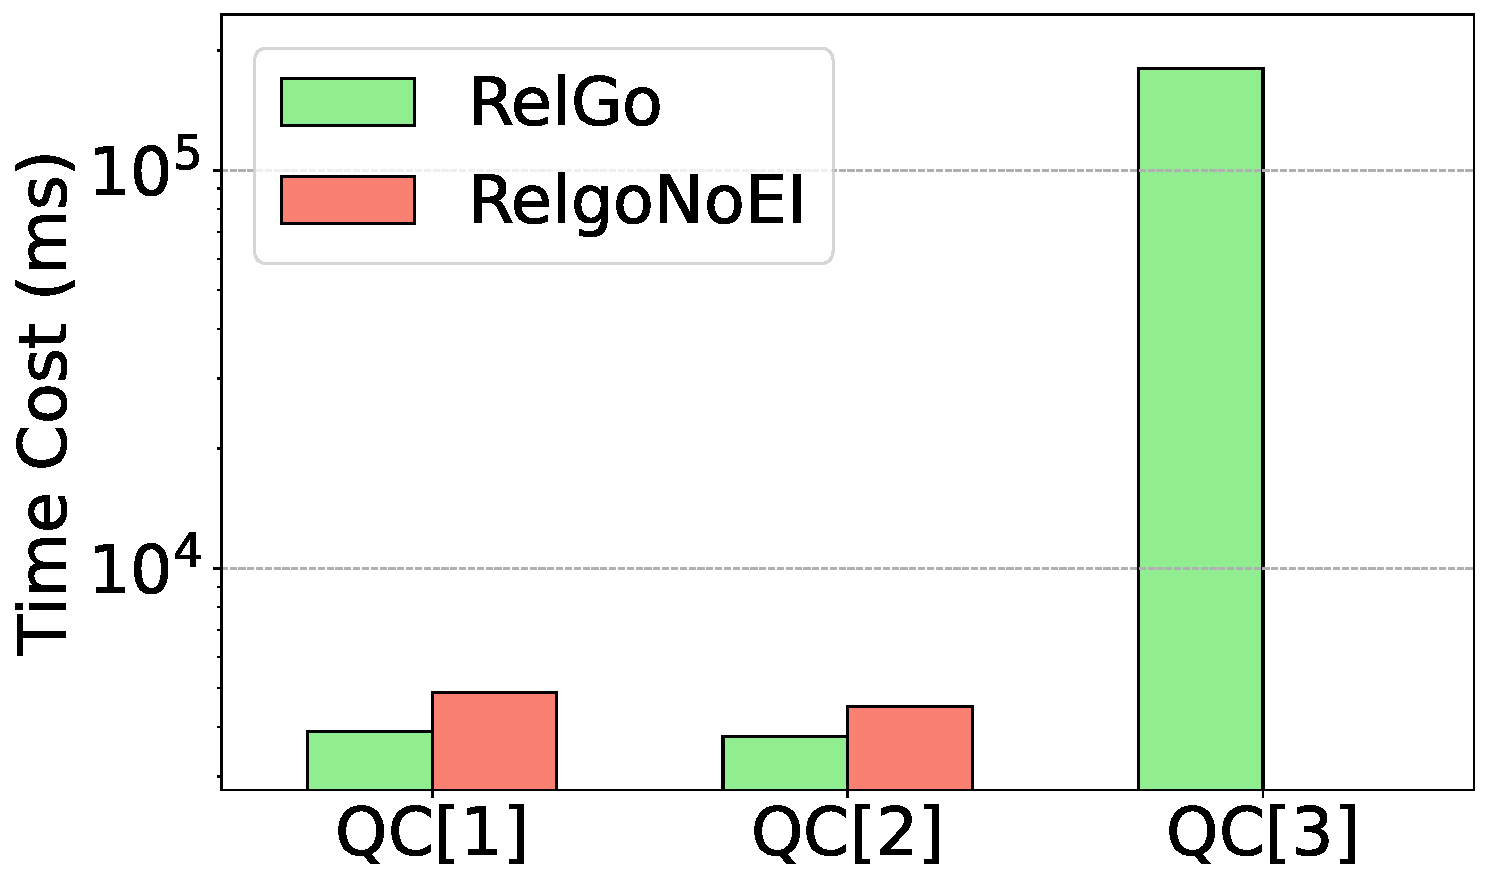
\includegraphics[width=\linewidth]{./figures/exp/ablation_ei_sf10.pdf}
        \vspace{-1.5em}
        \caption{Time Cost on $LDBC10$.}
        \label{fig:exp-expand-intersect-sf10}
    \end{subfigure}
    \begin{subfigure}[b]{0.45\linewidth}
        \centering
        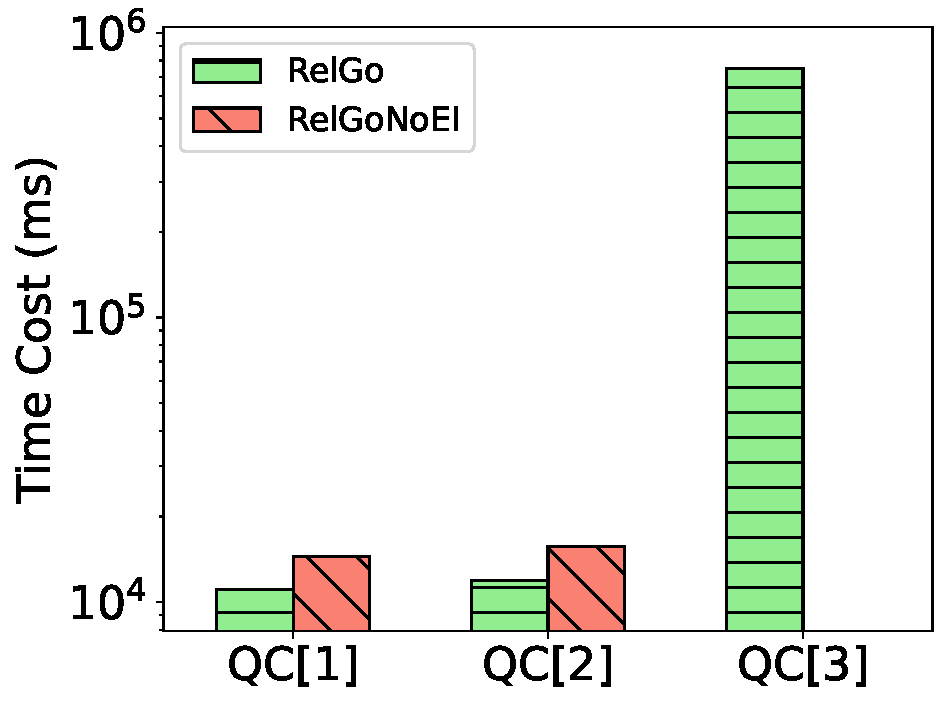
\includegraphics[width=\linewidth]{./figures/exp/ablation_ei_sf30.pdf}
        \vspace{-1.5em}
        \caption{Time Cost on $LDBC30$.}
        \label{fig:exp-expand-intersect-sf30}
    \end{subfigure}
    \caption{Efficiency comparison of \name and \relgomj}
    \label{fig:exp-expand-intersect}
\end{figure}


\noindent\textbf{Advanced Optimization Strategies.}
In this experiment, we assessed the advanced optimization strategies in \name, including the heuristic \filterrule and \joinfuserule, and the optimized implementation of \expandintersect~ operator that aims to improve the efficiency of complete star join.

We began by testing \filterrule and \joinfuserule, two representative heuristic rules employed in \name that capture optimization opportunities at the interplay of relational and graph optimizations. We conducted experiments on $LDBC10$ and $LDBC30$, using $QR[1]$ and $QR[2]$ to evaluate \filterrule, and $QR[3]$ and $QR[4]$ to test \joinfuserule. The results, depicted in \reffig{exp-filter}, compared the performance of \name with and without applying these rules, denoted as \name and \relgonofi, respectively.
The results demonstrate that \filterrule significantly improves query performance, providing an average speedup of 299.4$\times$ on $LDBC10$ and 699.8$\times$ on $LDBC30$. After applying \joinfuserule, query execution is accelerated by an average of 2.0$\times$ on $LDBC10$ and 2.3$\times$ on $LDBC30$. These findings suggest that the heuristic rules, particularly \filterrule, are highly effective in enhancing query execution efficiency.

%\enlargethispage{1em}

Next, we evaluated the effectiveness of the \expandintersect, which focuses on improving the efficiency of complete star join. Without this optimization strategy, the \expandintersect~ operator would be implemented as a traditional multiple join, and we denote this variant as \relgomj. We conducted this experiment with queries $QC[1 \ldots 3]$ that contain cycles and compared the performance of \name and \relgomj.
The performance results, depicted in \reffig{exp-expand-intersect}, suggest that, compared to \relgomj, \name achieves an average speedup of 1.22$\times$ on $LDBC10$ and 1.31$\times$ on $LDBC30$ (excluding $QC[3]$). Notably, for $QC[3]$, which is a complex 4-clique, the plans optimized by \relgomj confront an out-of-memory (OOM) error. %The reason is that applying worst-case optimal joins generates significantly fewer intermediate results than applying multiple joins, as numerous results that will not appear in the intersection are prematurely eliminated.
The results of this experiment indicate that the \expandintersect~ operator with an optimized implementation not only enhances query performance but also significantly reduces the spatial overhead.

\begin{figure}[ht]
    \centering
    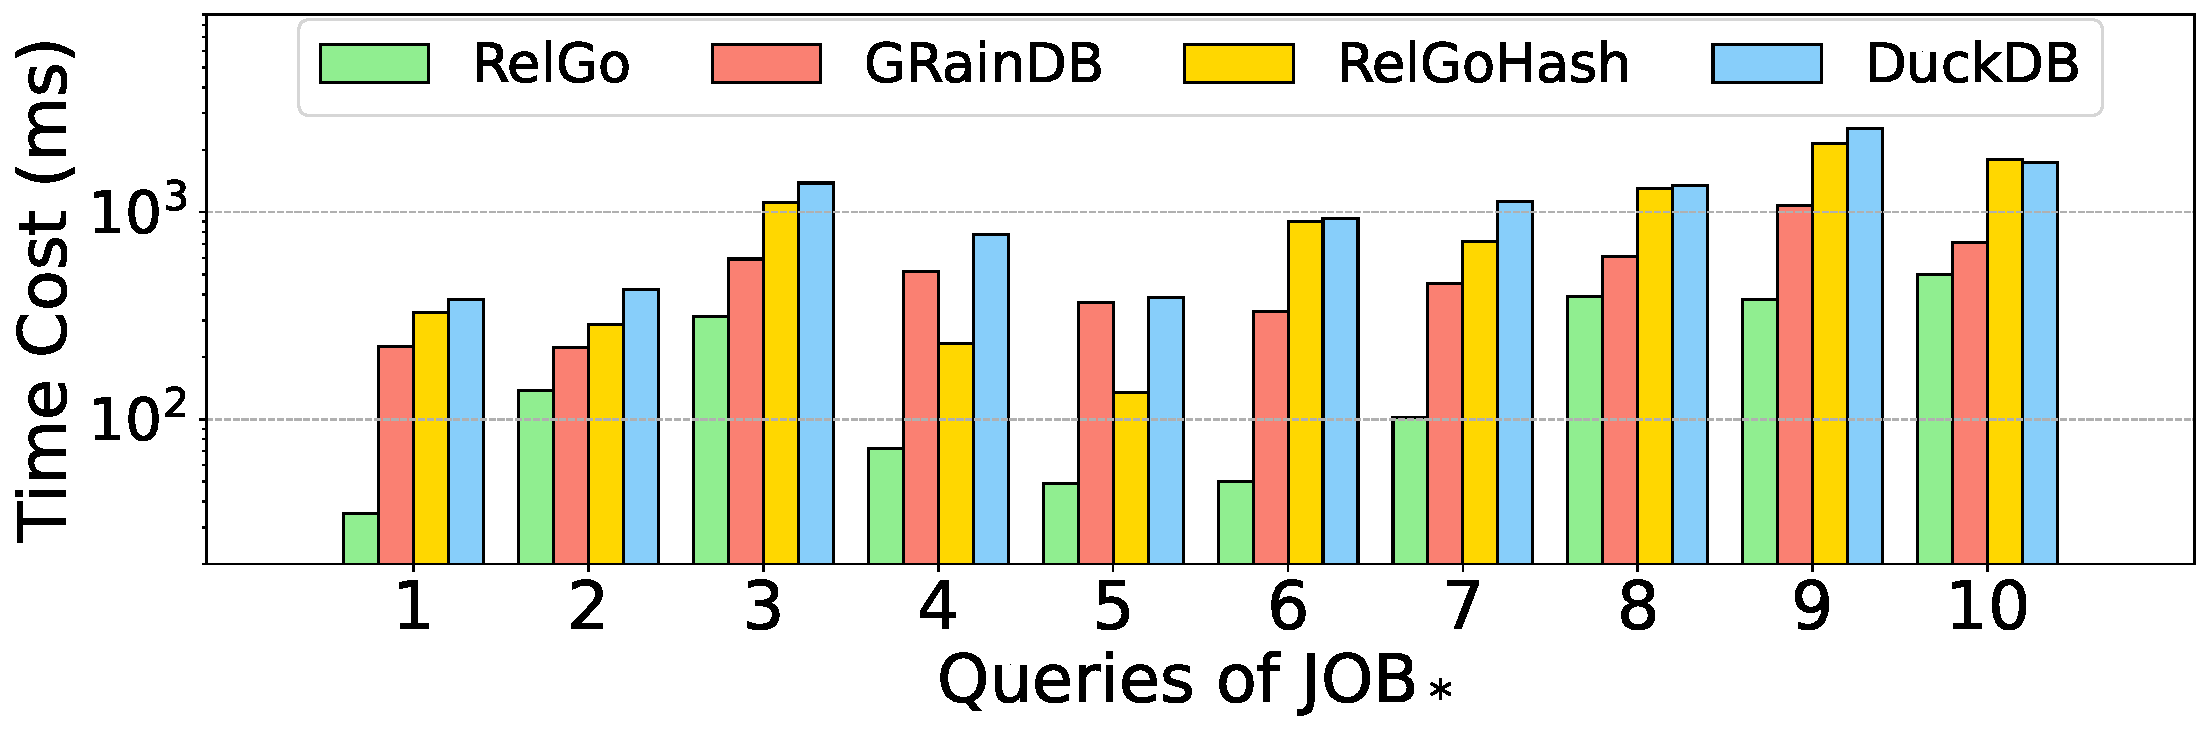
\includegraphics[width=\linewidth]{./figures/exp/hash_plan_job.pdf}
    \caption{Experiments on join order efficiency}
    \label{fig:exp-hash-plan}
\end{figure}

\noindent\textbf{Efficiency of Join Order.}
%After the assessment of advanced strategies within \name, we integrate all these strategies (and so as in the following experiments) to conduct a performance comparison between \name, GrainDB, and DuckDB with a focus on the join order efficiency.
In this experiment, we compared \name with GrainDB and DuckDB, focusing on the efficiency of the join order. For this purpose, we introduced a variant of \name called \relgohash, which optimizes the plan in a converged manner like \name but deliberately bypasses the use of graph index. We selected 10 queries from the JOB benchmark and showed the performance results in \reffig{exp-hash-plan}.
The results demonstrate that \name outperforms GrainDB on all the queries, accelerating the execution time by factors ranging from \revise{$1.4\times$} to $7.5\times$, with an average speedup of \revise{$4.14\times$}. Additionally, the plans optimized with \relgohash are at least as good as those optimized by DuckDB, achieving an average speedup of \revise{$1.6\times$}. The effectiveness of \name and \relgohash stems from their use of advanced graph-aware optimization techniques in optimizing the matching operator, resulting in good join order and thus robust performance regardless of the presence or absence of graph index.
It is worth noting that \name does not always generate plans with the absolute best join orders, as it relies on the estimated cost of the plans. However, its optimized plans generally remain competitive in most cases, thanks to its integration of \glogue that use high-order statistics for cost estimation.

%This superior join order offsets the absence of graph indices in the execution process.

% In this section, we conduct ablation study to show the efficiency of \expandintersectrule.
% In detail, patterns in Fig.~\ref{fig:exp-hard-patterns} are queried on $LDBC10$ and $LDBC30$, and plans are optimized with Relgo.
% For each plan optimized by Relgo, we replace the extend-intersect operators in it with multiple join operators and obtain a new plan.
% These new plans are called obtained with \textit{"Relgo w.o. EI"}.
% The experimental results are shown in Fig.~\ref{fig:exp-ablation-ei}.

% The results illustrate the efficiency of \expandintersectrule.
% When triangles are searched for, removing the extend-intersect operators decreases the query performance.
% Besides, when butterflies and 4-cliques are searched for, the plans without extend-intersect operators have an excessive memory overhead and cause an ``Out of Memory'' (abbr.~OOM) error.
% The reason is that applying extend-intersect operators has much fewer intermediate results than applying multiple joins, since numerous results that will not appear in the intersection are prematurely deleted.
% It indicates that \expandintersectrule can not only enhance query performance, but also reduce spatial overhead.

% To further demonstrate the efficiency of \expandintersectrule, we add predicates on butterflies (i.e., Fig.~\ref{fig:exp-hard-butterfly}) and 4-cliques (i.e., Fig.~\ref{fig:exp-hard-clique}) to avoid OOM, and generate two new patterns, i.e., \textit{Butterfly-P} and \textit{4-Clique-P}.
% Specifically, for these two new patterns, the values of properties Person1.\textit{p\_personid} are constrained to be smaller than specified values.
% Queries of these new patterns are optimized with GrainDB, \name, and \textit{\name w.r. EI}.
% The results on the constrained-patterns are shown in Fig.~\ref{fig:exp-ablation-para-ei}.


% The results suggest that \expandintersectrule is crucial in optimizing queries with cycles.
% Specifically, for the new patterns with cycles, the execution time of plans optimized by \name is more than an order of magnitude shorter than those optimized by \textit{"Relgo w.o. EI"}.
% It indicates the effectiveness of \expandintersectrule.
% Moreover, when patterns with many cycles are used (e.g., 4-clique in Fig.~\ref{fig:exp-hard-clique}), the optimization effect of the rule becomes particularly noticeable.
% In detail, querying for 4-cliques with \name can be 100$\times$ faster than with \textit{"Relgo w.o. EI"}.
% The results illustrate the efficiency of \expandintersectrule.

\begin{figure}[ht]
    \centering
    \begin{subfigure}[b]{\linewidth}
        \centering
        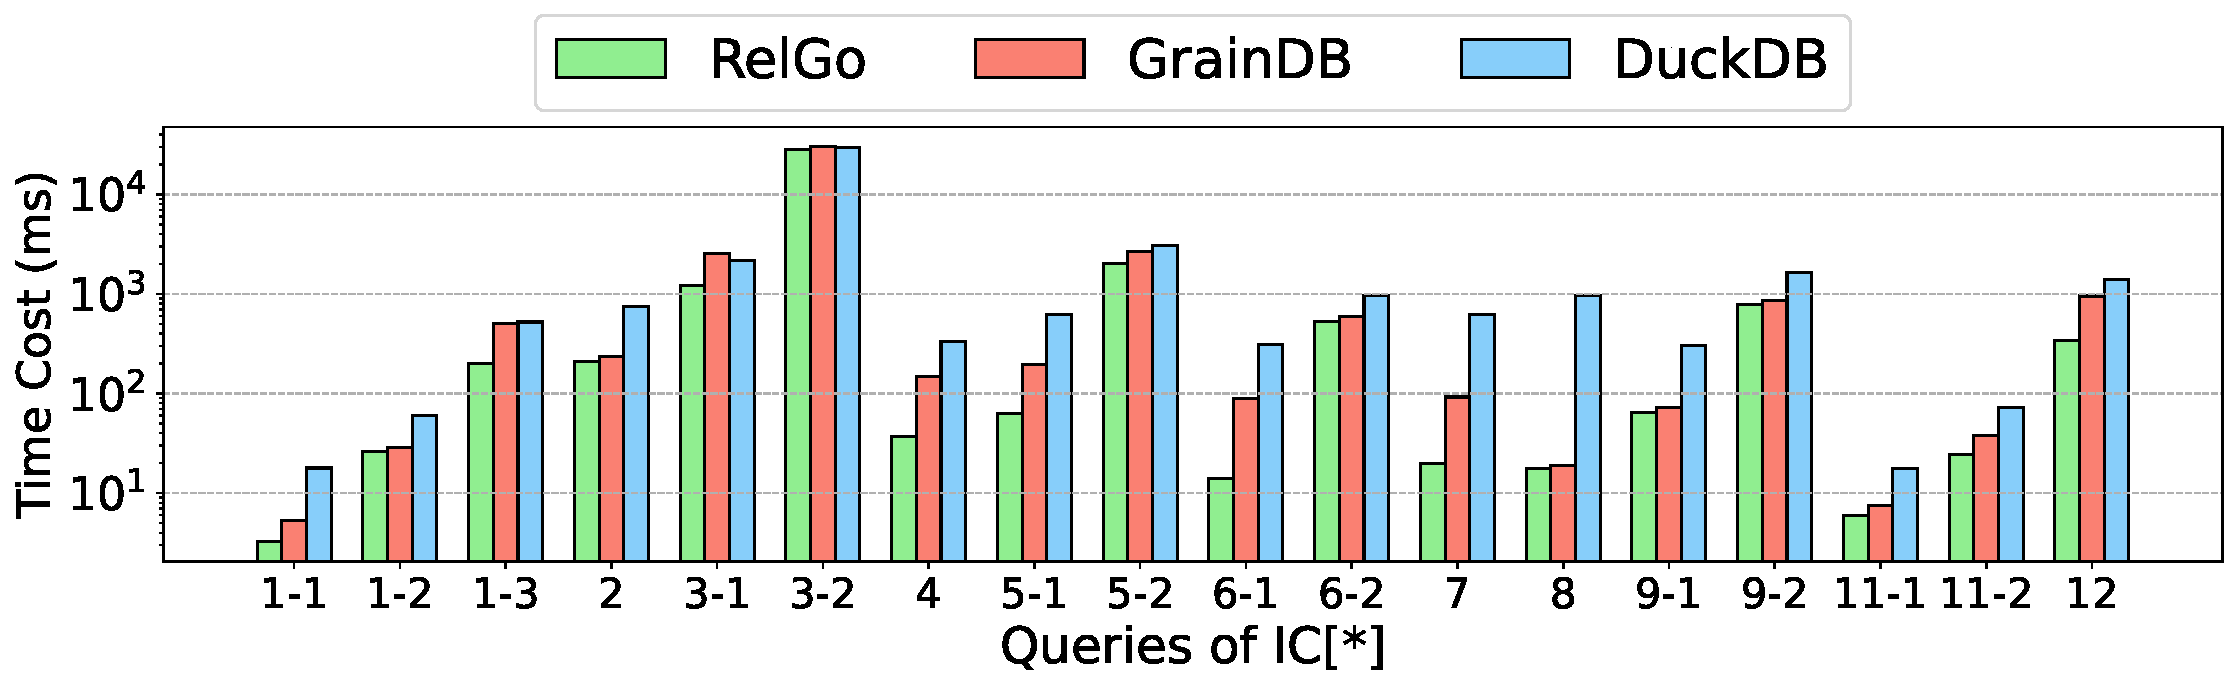
\includegraphics[width=\linewidth]{./figures/exp/e2e_sf10.pdf}
        \vspace{-2em}
        \caption{Speedup Compared to DuckDB on $LDBC10$.}
        \label{fig:exp-e2e-sf10}
    \end{subfigure}
    \begin{subfigure}[b]{\linewidth}
        \centering
        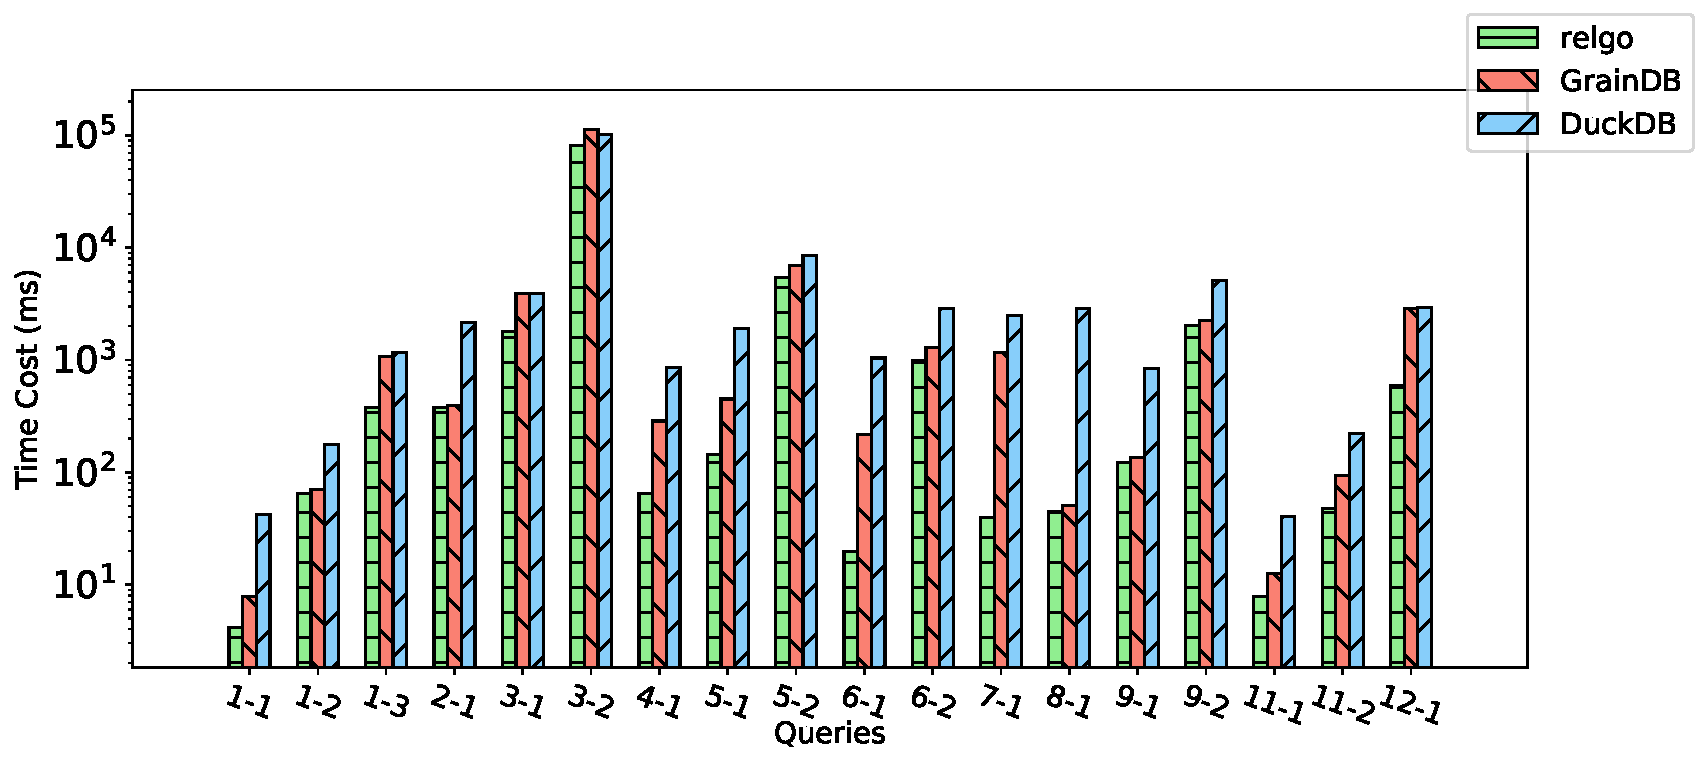
\includegraphics[width=\linewidth]{./figures/exp/e2e_sf30.pdf}
        \vspace{-2em}
        \caption{Speedup Compared to DuckDB on $LDBC30$.}
        \label{fig:exp-e2e-sf30}
    \end{subfigure}
    \begin{subfigure}[b]{\linewidth}
        \centering
        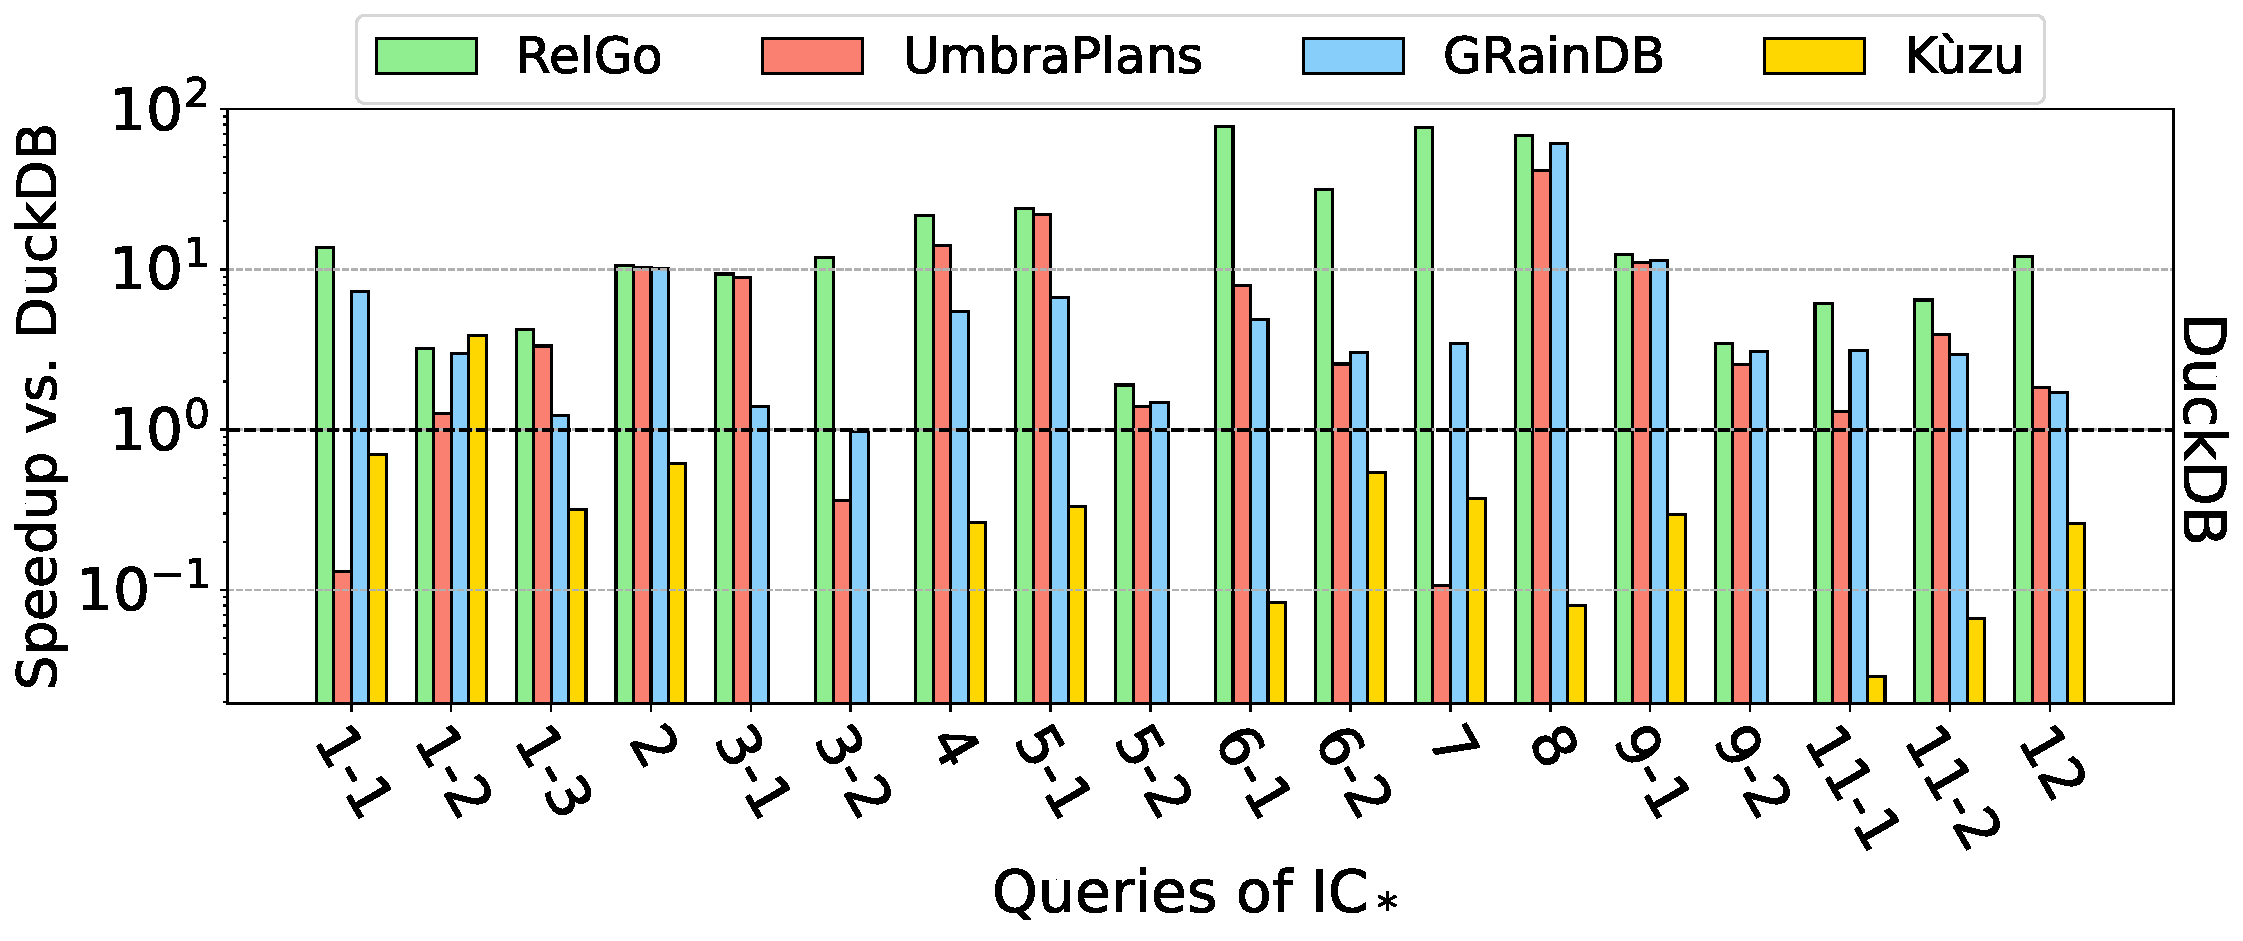
\includegraphics[width=\linewidth]{./figures/exp/e2e_sf100.pdf}
        \vspace{-2em}
        \caption{Speedup Compared to DuckDB on $LDBC100$.}
        \label{fig:exp-e2e-sf30}
    \end{subfigure}
    \begin{subfigure}[b]{\linewidth}
        \centering
        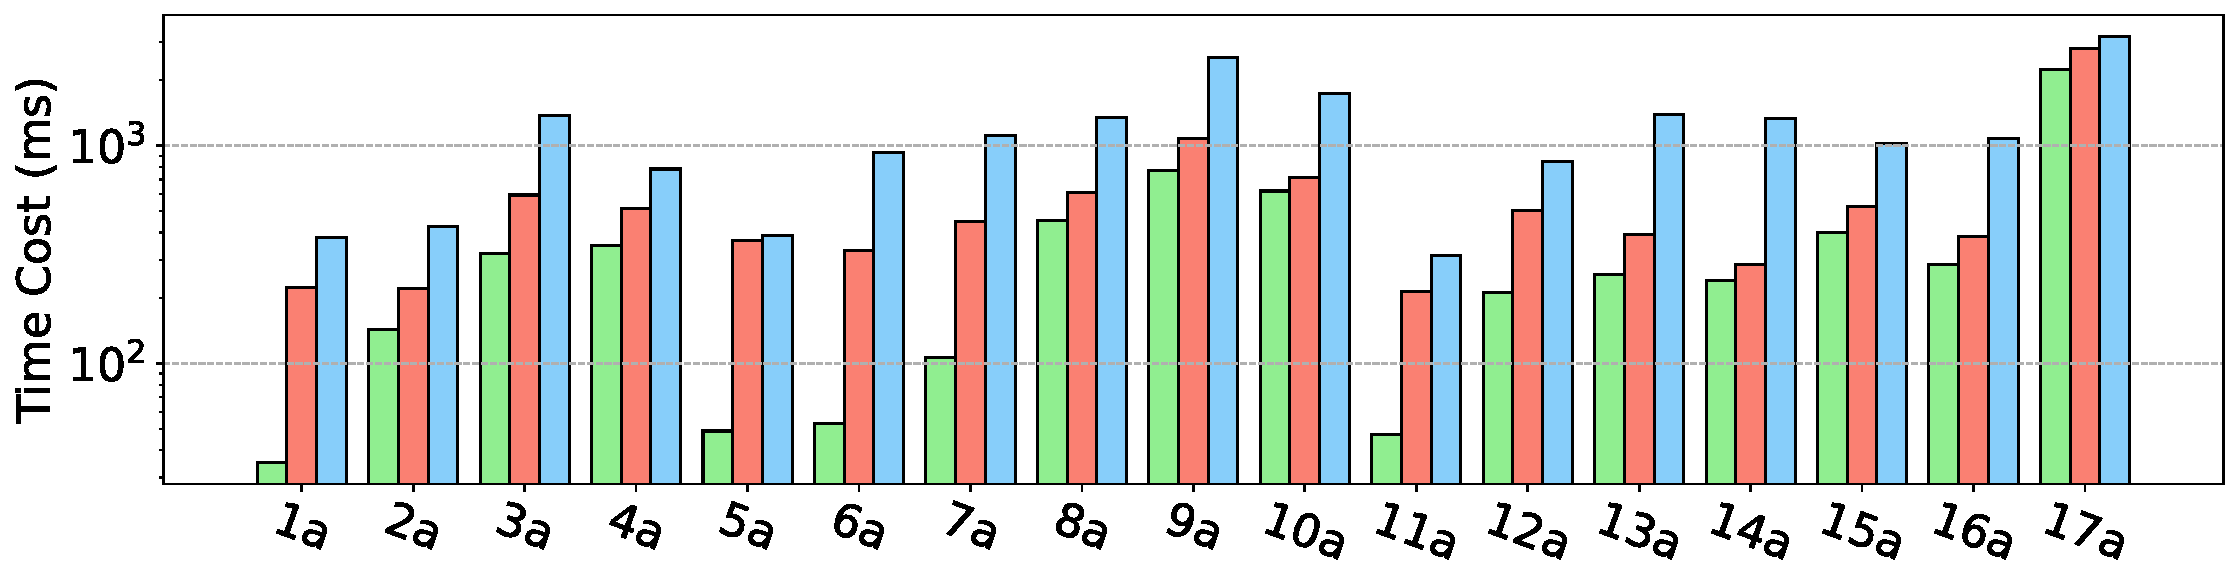
\includegraphics[width=\linewidth]{./figures/exp/e2e_job_part1.pdf}
        \vspace*{-2ex}
    \end{subfigure}
    \begin{subfigure}[b]{\linewidth}
        \centering
        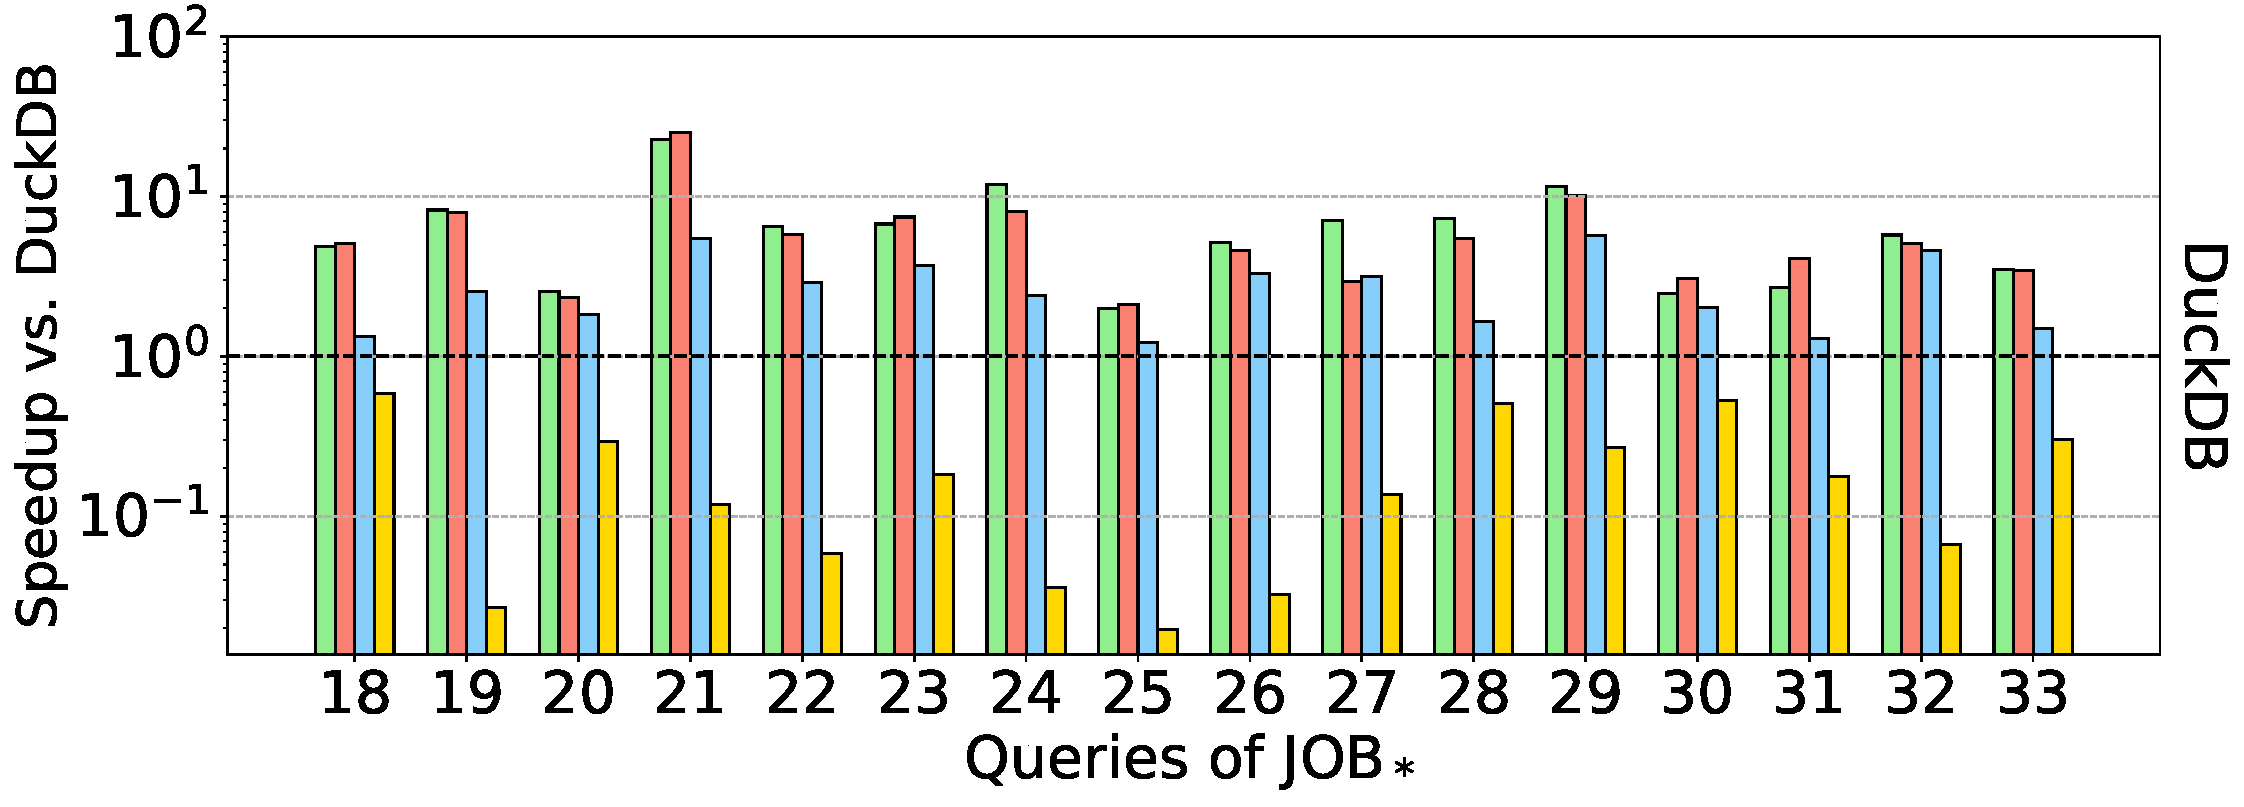
\includegraphics[width=\linewidth]{./figures/exp/e2e_job_part2.pdf}
        \vspace{-2em}
        \caption{Speedup Compared to DuckDB on IMDB.}
        \label{fig:exp-e2e-job}
    \end{subfigure}
    \caption{Results of the comprehensive experiments. The speedup of method A compared to DuckDB is computed as $\frac{\text{Time}(DuckDB)}{\text{Time}(A)}$. Note that the results of K\`uzu are sometimes omitted (e.g., IC[3-1] and IC[3-2] on $LDBC10$) due to out-of-memory errors (abbr.~OOM).}
    \label{fig:exp-e2e}
\end{figure}

\subsection{Comprehensive Experiments}
\label{sec:experiment-e2e}

We conducted comprehensive experiments on the LDBC and JOB benchmarks to comprehensively evaluate the performance of \name compared to \revise{the baselines, i.e., DuckDB, GrainDB, Umbra, and K\`uzu}. The experimental results, presented in \reffig{exp-e2e}, demonstrate that execution plans optimized by \name consistently \revise{outperform those optimized by the baselines on both benchmarks}.

\subsubsection{Comparison with DuckDB and GrainDB}

Firstly, we compare the performance of \name with DuckDB and GrainDB.
Specifically, for the LDBC benchmark, the execution time of the plans optimized by \name is about \revise{12.4$\times$} and \revise{5.0$\times$} faster on average than those generated by DuckDB and GrainDB on $LDBC10$, about \revise{17.9$\times$} and \revise{6.6$\times$} on $LDBC30$, and about 21.9$\times$ and 5.4$\times$ on $LDBC100$.
It is important to note that \name is especially effective for queries containing cycles, which can benefit more from graph optimizations. For example, in query $IC[7]$, which contains a cycle, \name outperforms DuckDB and GrainDB by \revise{63.5$\times$ and 29.7$\times$}, respectively, on $LDBC30$.
Conversely, the JOB benchmark, established for assessing join optimizations in relational databases, lacks any cyclic-pattern queries. Despite this, \name still achieves better performance compared to DuckDB and GrainDB, with an average speedup of 8.2$\times$ and 4.0$\times$, respectively.

The experimental results reflect our discussions in \refsec{graph-aware}. We summarize the superiority of \name as follows.
First, \name is designed to be aware of the existence of graph index in query optimization and can leverage the index to effectively retrieve adjacent edges and vertices. In contrast, for \revise{GrainDB}, relational optimizers can occasionally alter the order of \EVjoin operations, rendering graph index ineffective. DuckDB, on the other hand, does not consider graph index in query optimization and executes queries using conventional hash joins, which are often less efficient compared to graph-aware approaches.
Second, by incorporating a matching operator in \spjm queries to capture the graph query semantics, \name is able to leverage advanced graph optimization techniques to optimize the matching operator. These techniques include using high-order statistics to estimate the cost of plans more accurately and employing worst-case optimal join implementations to optimize cyclic patterns. In contrast, DuckDB and GrainDB cannot benefit from these graph-specific optimizations, which may lead to suboptimal plans and inefficient execution.
Third, \name considers optimization opportunities across both graph and relational query semantics, introducing effective heuristic rules such as \filterrule and \joinfuserule. These rules can significantly improve the efficiency of the generated plans.


\subsubsection{Comparsion with Umbra}
Then, we compare the performance of \name and Umbra according to the experimental results presented in \reffig{exp-e2e}.
In detail, the plans optimized by \name are about \revise{22.4$\times$, 37.6$\times$, and 49.9$\times$} faster on average than those generated by Umbra on $LDBC10$, $LDBC30$, and $LDBC100$, respectively.
On JOB benchmark, which is a traditional relational workload, the plans generated by \name are, on average, 1.7$\times$ more efficient than those generated by Umbra.
The following reasons primarily contribute to this improvement:
(1) Umbra, due to its lack of a graph perspective, might generate query plans that could encounter issues in using the graph indexes similarly to GrainDB.
(2) Although Umbra's optimizer supports generating execution plans that include multiway joins, in our actual experiments, none of the optimized plans for the queries contained multiway joins. This indicates that Umbra also struggles to leverage the graph-specific optimizations

Notably, \revise{there are instances where Umbra generates better execution plans compared to \name, e.g., when JOB[30] is queried on IMDB, the execution time of the plan generated by \name is about 1.2$\times$ that of Umbra. A possible reason is that the distributions of attribute values are not yet considered in \name and the Umbra can sometimes estimate cardinalities more accurately when predicates exist.
We consider this as our further work}.


\subsubsection{Comparison with K\`uzu}
Finally, we compare \name with the widely used GDBMS, i.e., K\`uzu.
The experimental results in \reffig{exp-e2e} show that \name is about \revise{77.4$\times$}, \revise{125.9$\times$} and \revise{188.7$\times$} faster on average than K\`uzu on $LDBC10$, $LD BC30$ and $LDBC100$, respectively.
Besides, \name achieves an average speedup of 136.1$\times$ compared to K\`uzu on the JOB benchmark.
This indicates that \name, when using DuckDB as the execution engine, can achieve even better performance than GDBMS like K\`uzu.
This may be because the index used in Kuzu is less efficient than ours.





% There are mainly two reasons for the superiority of \name.
% Firstly, \name is aware of the existence of graph indices in graph query optimization.
% Thus, the cost estimation of \name is more accurate and better physical plans can be obtained.
% In contrast, the optimizers of DuckDB and GrainDB are of the types $Rel$ and $Rel^+$, respectively, and are not aware of the graph indices in query optimization phase.
% Therefore, the accuracy of cost estimation is limited.
% Secondly, for queries with cycles (e.g., $IC[7]-1$ on LDBC), \name have a superior performance due to the advanced extend-intersect operators, which outperforms the traditional multiple join operators used by DuckDB and GrainDB.
% Such an operator can significantly reduce the time consumption, which is also demonstrated through experiments in \reffig{exp-expand-intersect}.
% \todo{update this, with the new TrimFusionRule:} Thirdly, \name is more adept at identifying opportunities to effectively utilize graph indices to get neighbors of vertices, since it optimizes graph queries from the graph perspective.
% Conversely, GrainDB occasionally partitions the process into separate stages, first retrieving adjacent edges and subsequently obtaining the corresponding endpoints.

\begin{figure}[ht]
    \centering
    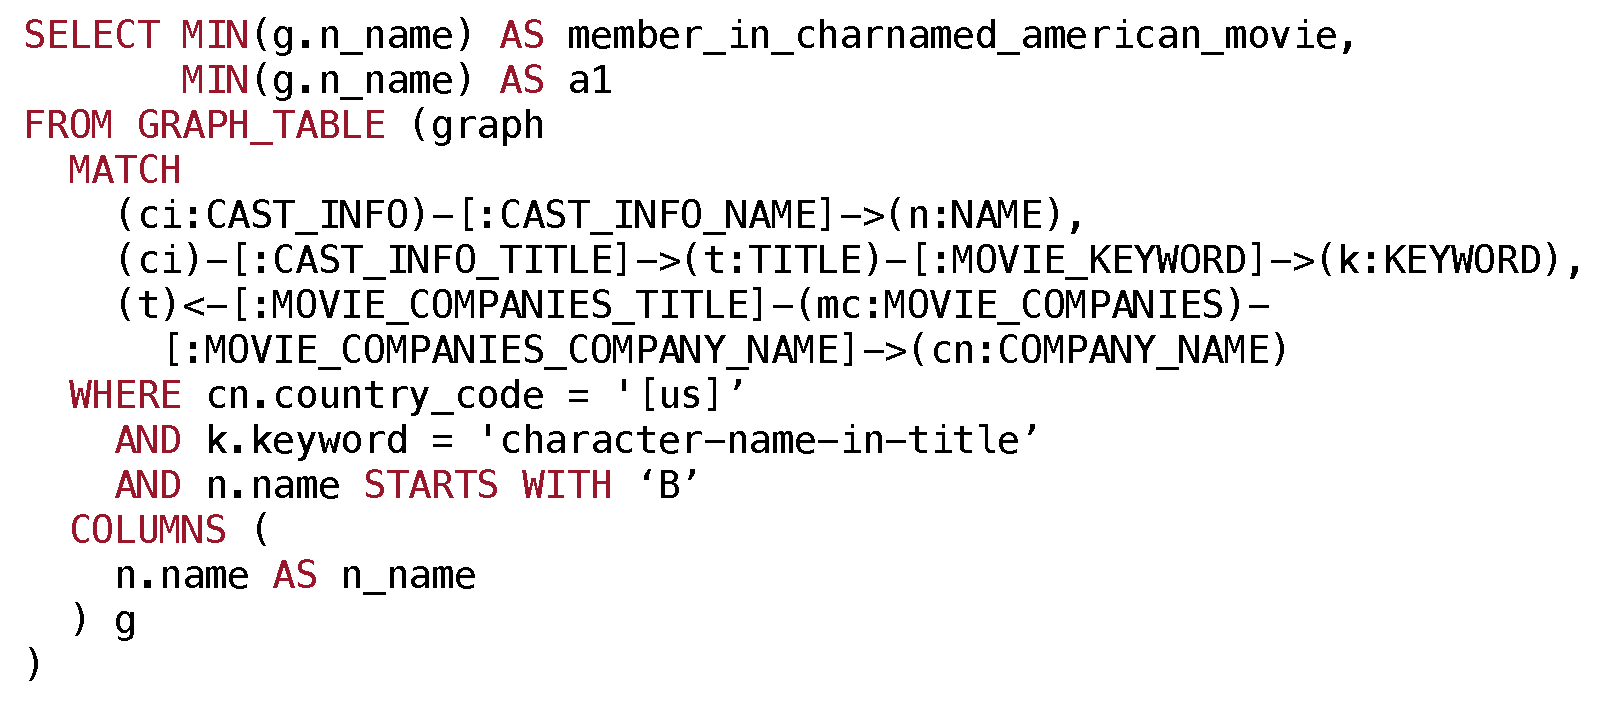
\includegraphics[width=\linewidth]{./figures/job17a-query.pdf}
    \caption{JOB[17] query.}
    \label{fig:job17-query}
\end{figure}


\begin{figure*}[ht]
    \centering
    \begin{subfigure}[b]{.3\linewidth}
        \centering
        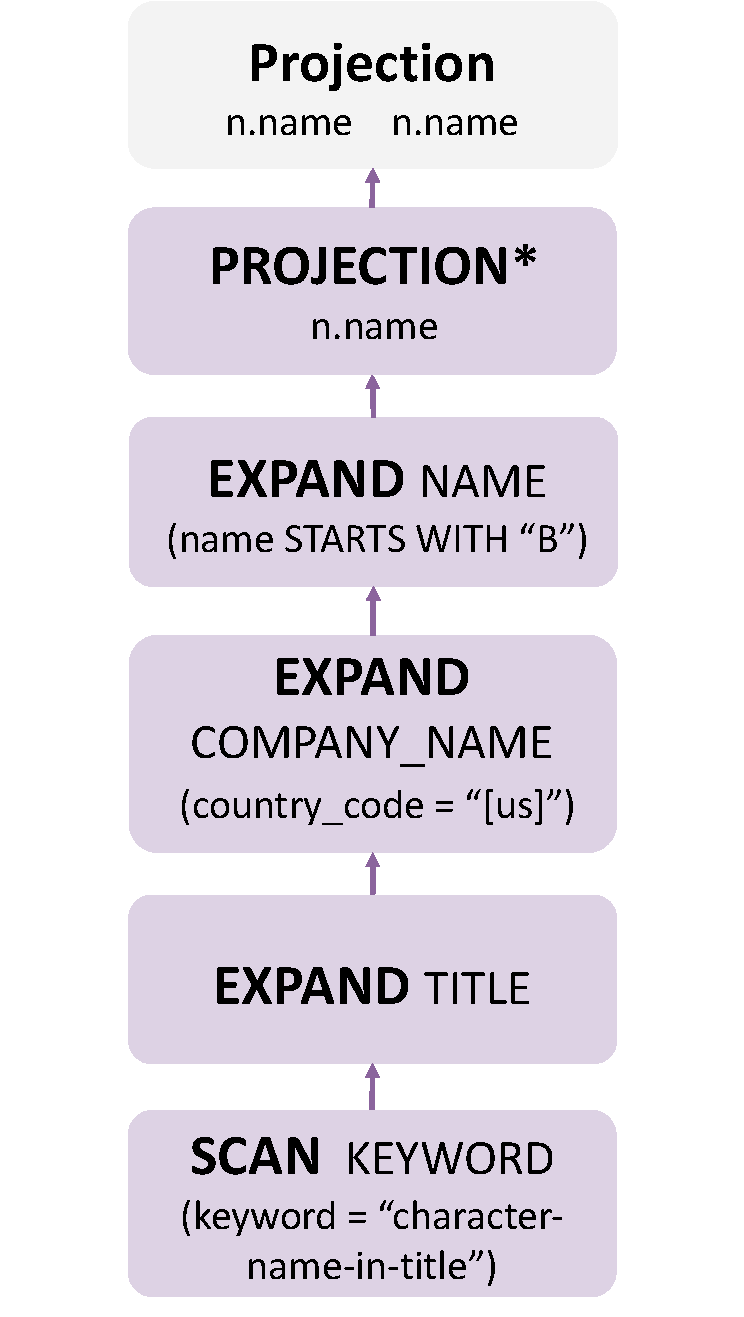
\includegraphics[width=.5\linewidth]{./figures/job17a-plan-gopt.pdf}
        \caption{Query Plan of \name.}
        \label{fig:job17a-plan-relgo}
    \end{subfigure}
    \begin{subfigure}[b]{.25\linewidth}
        \centering
        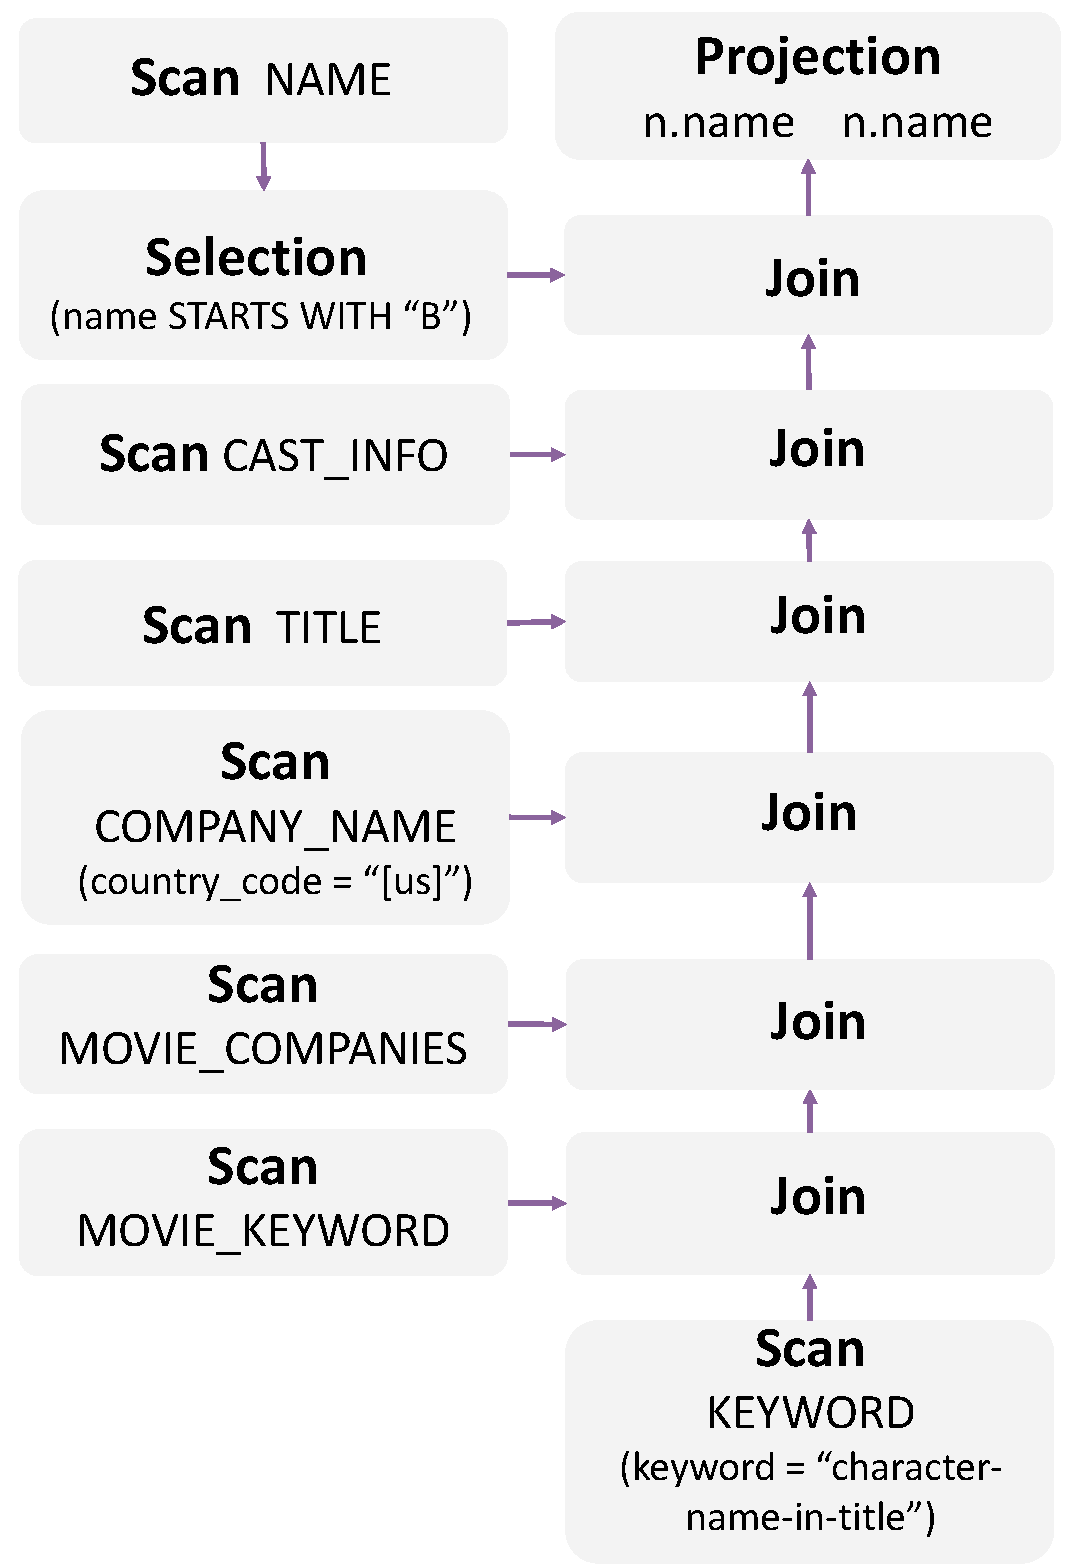
\includegraphics[width=.85\linewidth]{./figures/job17a-plan-graindb.pdf}
        \caption{Query Plan of GrainDB.}
        \label{fig:job17a-plan-graindb}
    \end{subfigure}
    \begin{subfigure}[b]{.4\linewidth}
        \centering
        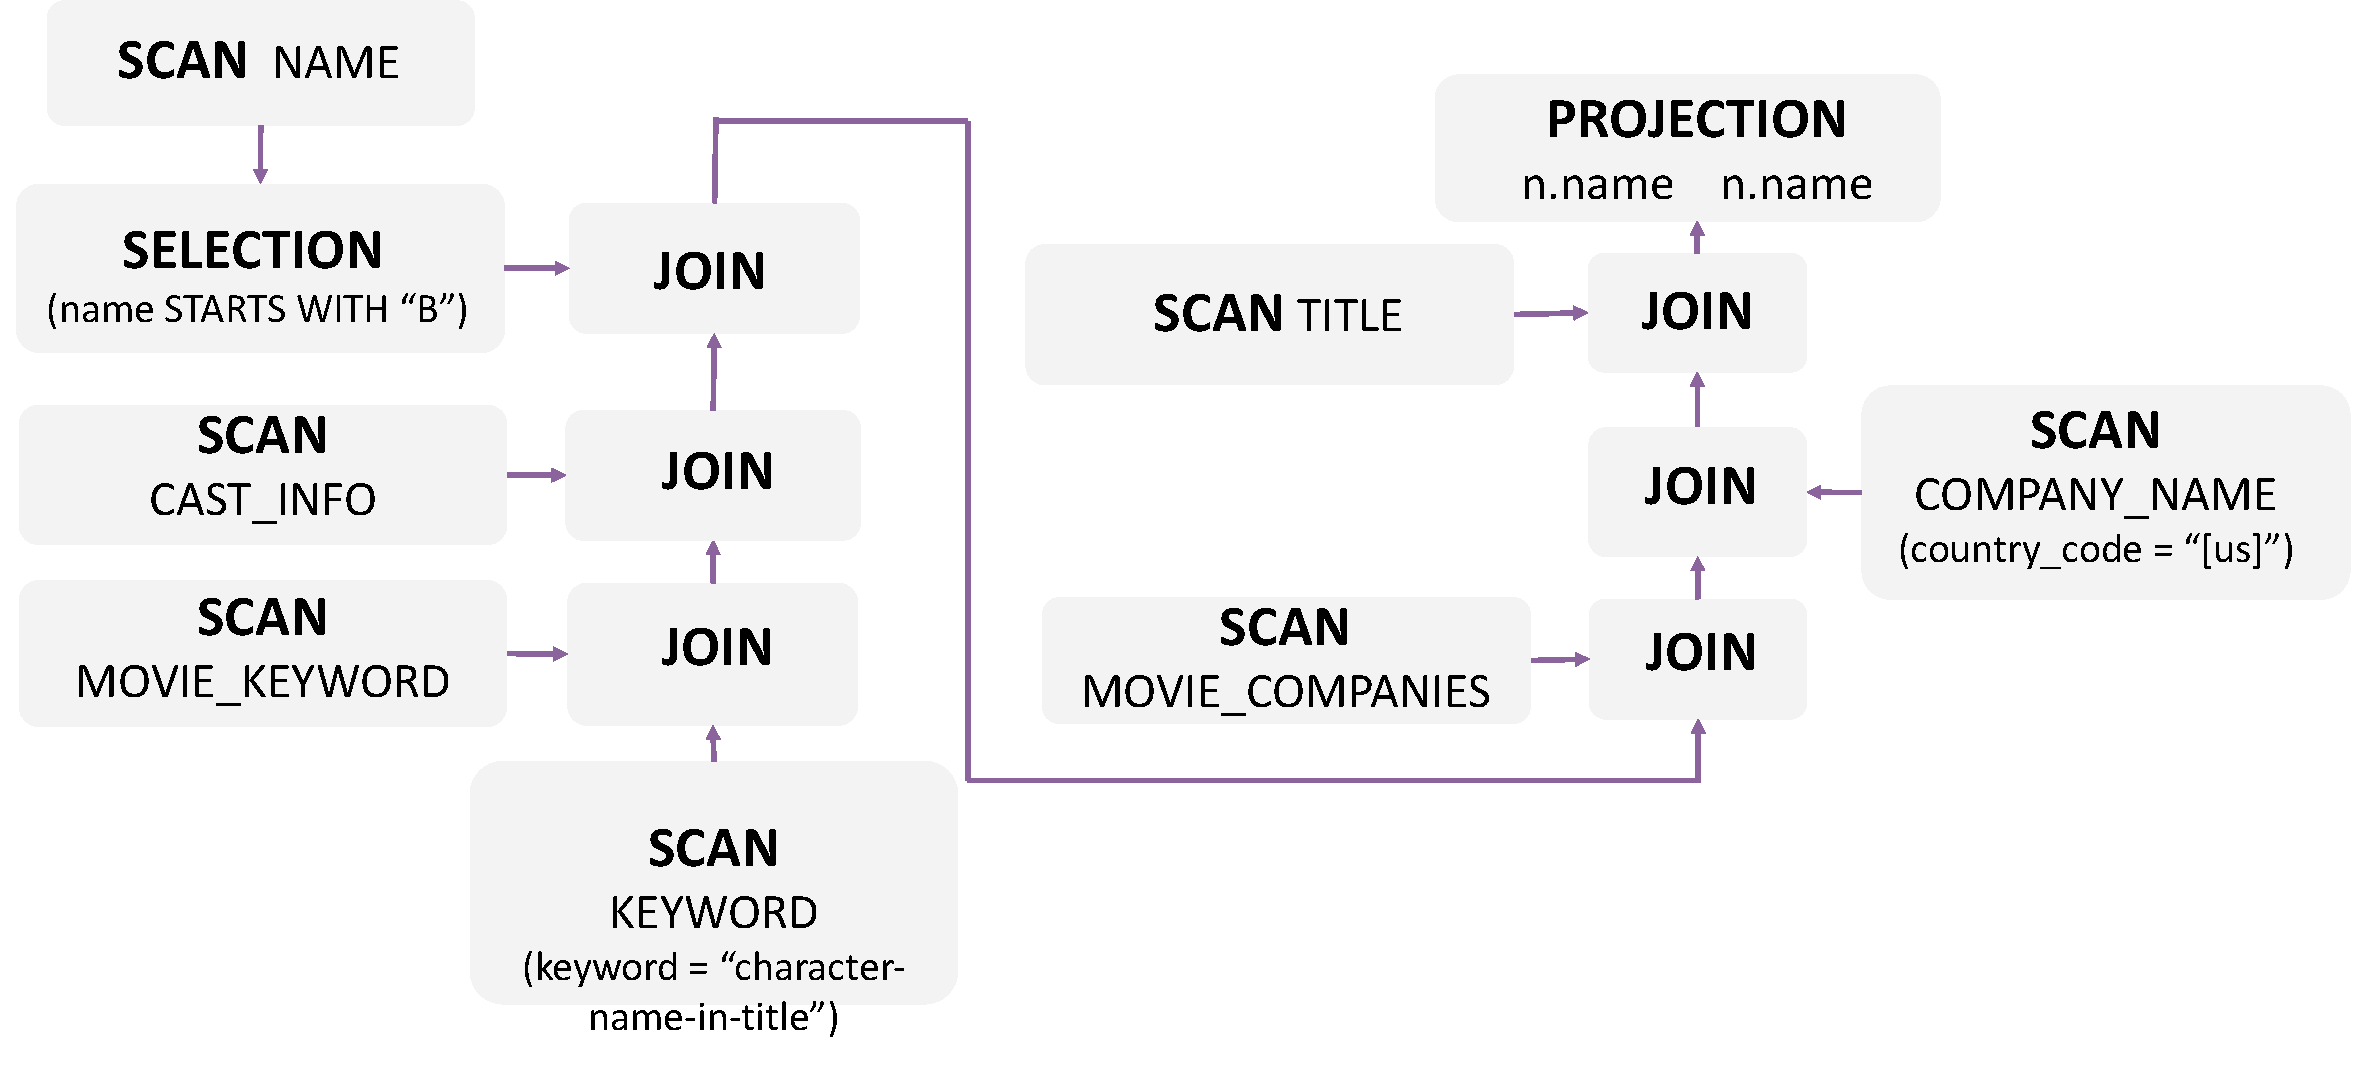
\includegraphics[width=.9\linewidth]{./figures/job17a-plan-umbra.pdf}
        \caption{Query Plan of Umbra}
        \label{fig:job17a-plan-umbra}
    \end{subfigure}
    \caption{\revise{Query plans of JOB[17] generated by \name, GrainDB, and Umbra.}}
    \label{fig:job17a-query-plans}
\end{figure*}


\subsection{Case Study}
\revise{To further illustrate why the plans generated by \name are better than those generated by the baseline optimizers, we conduct a case study using the JOB[17] query as an example.
The query is shown in \reffig{job17-query}.
Specifically, the query plans optimized by \name, GrainDB, and Umbra for this query are shown in \reffig{job17a-query-plans}}.


The \revise{plan of \name starts from $\relation{\text{keyword}}$.
According to the plan, the results of scanning $\relation{\text{keyword}}$ expand to $\relation{\text{title}}$, $\relation{\text{company\_name}}$, and $\relation{\text{\name}}$ in sequence.
Please note that when $\mathcal{P}_{\name}$ expands from $\relation{\text{keyword}}$ to $\relation{\text{title}}$, an \expandedge~ operator followed by \getvertex~ operator is generated.
Then, \joinfuserule~ is applied to merge these two operators into an \expand~ operator.
The \expand~ operator is implemented as a predefined join utilized in GrainDB that efficiently retrieve the neighboring vertices based on the VE-index}.

However, \revise{because GrainDB and Umbra apply relational optimizers, it is not necessary for them to join vertex relations and edge relations alternately. Consequently, they may miss opportunities to achieve better execution plans using the \joinfuserule, and cannot merge join operators such as $\relation{\text{keyword}} \bowtie \relation{\text{movie\_keyword}}$ and $\relation{\text{movie\_keyword}} \bowtie \relation{\text{title}}$}.

Moreover, \revise{the advantage of \name over baseline optimizers also stems from its support for the \expandintersect~ operation. For instance, given the IC[7] query, the execution plan generated by \name includes an EI-Join. This provides a significant advantage over the plans optimized by other optimizers}.
